\section{Edge\-Xover Class Reference}
\label{class_edge_xover}\index{EdgeXover@{EdgeXover}}
Edge Crossover.  


{\tt \#include $<$edge\_\-xover.h$>$}

Inheritance diagram for Edge\-Xover::\begin{figure}[H]
\begin{center}
\leavevmode
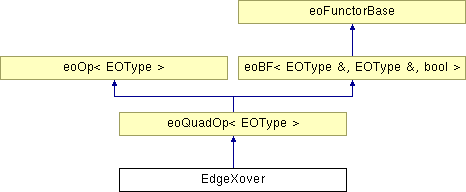
\includegraphics[height=4cm]{class_edge_xover}
\end{center}
\end{figure}
\subsection*{Public Member Functions}
\begin{CompactItemize}
\item 
bool \bf{operator()} (\bf{Route} \&\_\-\_\-route1, \bf{Route} \&\_\-\_\-route2)\label{class_edge_xover_cb1c0a103106a4d3319540cb23163a79}

\end{CompactItemize}
\subsection*{Private Member Functions}
\begin{CompactItemize}
\item 
void \bf{cross} (const \bf{Route} \&\_\-\_\-par1, const \bf{Route} \&\_\-\_\-par2, \bf{Route} \&\_\-\_\-child)\label{class_edge_xover_88c2d4c9a878454a32d56010f3dddc27}

\item 
void \bf{build\_\-map} (const \bf{Route} \&\_\-\_\-par1, const \bf{Route} \&\_\-\_\-par2)\label{class_edge_xover_04de96aa1016836e0ba5f4b952a5fa16}

\item 
void \bf{add\_\-vertex} (unsigned int \_\-\_\-vertex, \bf{Route} \&\_\-\_\-child)\label{class_edge_xover_b590458c35c16a14896a4bcdf9674ade}

\end{CompactItemize}
\subsection*{Private Attributes}
\begin{CompactItemize}
\item 
std::vector$<$ std::set$<$ unsigned int $>$ $>$ \bf{\_\-map}\label{class_edge_xover_7d9272c12cfa55df4677d5ad837a0e5c}

\item 
std::vector$<$ bool $>$ \bf{visited}\label{class_edge_xover_46d4d4724cf6d660b1a7ab4a346573d4}

\end{CompactItemize}


\subsection{Detailed Description}
Edge Crossover. 



Definition at line 48 of file edge\_\-xover.h.

The documentation for this class was generated from the following files:\begin{CompactItemize}
\item 
edge\_\-xover.h\item 
edge\_\-xover.cpp\end{CompactItemize}
